% nmedoc.tex V3.01, 2 March 2016

\documentclass[times]{nmeauth}

\usepackage{moreverb}


\usepackage[colorlinks,bookmarksopen,bookmarksnumbered,citecolor=red,urlcolor=red]{hyperref}

\usepackage{undertilde}

\newcommand\BibTeX{{\rmfamily B\kern-.05em \textsc{i\kern-.025em b}\kern-.08em
T\kern-.1667em\lower.7ex\hbox{E}\kern-.125emX}}

\def\volumeyear{2016}

\begin{document}

\runningheads{T.~Martin}{One-Dimensional Uncoupled Thermoelastic Response of Spherical Pressure Vessel}
%\runningheads{T.~Martin}{A demonstration of the \journalabb\
%class file}

%\title{A demonstration of the \LaTeXe\ class file for the
%\itshape{\journalnamelc}\footnotemark[2]}
\title{One-Dimensional Uncoupled Thermoelastic Response of a Spherical Pressure Vessel to an Internal Wall Heat Source}
\author{Tony Martin\corrauth\affil{1}}

\address{John Wiley \& Sons, Ltd, The Atrium, Southern Gate, Chichester,
West Sussex, PO19~8SQ, UK}

\corraddr{Journals Production Department, John Wiley \& Sons, Ltd,
The Atrium, Southern Gate, Chichester, West Sussex, PO19~8SQ, UK.}

\begin{abstract}
This paper describes the procedure for numerically analyzing the thermal and mechanical response of a spherical pressure vessel to an increase in temperature on the inner surface. The pressure vessel is subject to a heat source at the inner surface, and at some time the temperature is increased according to some function. The increase in temperature result in expansion of the two materials that make up the pressure vessel wall. This type of analysis is also known as a thermoelastic analysis (or uncoupled thermoelasticity), where thermal effects within the material enter the material as a body force. It was seen that through finite differencing methods, this analysis can be readily accomplished for any material.  
%This paper describes the use of the \LaTeXe\
%\textsf{\journalclass} class file for setting papers for the
%\emph{\journalnamelc}.
\end{abstract}

\keywords{Heat Diffusion, Radial Stress, Hoop Stress, Thermoelasticity; \LaTeXe; \emph{\journalabb}}

\maketitle

\footnotetext[2]{Please ensure that you use the most up to date
class file,
available from the NME Home Page at\\
\href{http://onlinelibrary.wiley.com/journal/10.1002/(ISSN)1097-0207}{\texttt{http://onlinelibrary.wiley.com/journal/10.1002/(ISSN)1097-0207}}}

\vspace{-6pt}

\section{Introduction}
\vspace{-2pt}
The one-dimensional heat equation for spherical coordinates is used to calculate the thermal response of a spherical pressure vessel to a heat source located at the inner surface. The one-dimensional displacement equation is also used to determine the displacements throughout the vessel, along with the resulting radial and Hoop stresses. The analysis is done by implementing finite difference techniques. For the thermal solution, an implicit method is used, where the current temperature can only be solved using the temperature at from the previous time step. This results in a system of linear equations that can only be solved by inverting matrices. Matlab is utilized to implement these finite difference methods and invert the matrices to converge to a solution. Throughout the analysis, either centered differencing, forward differencing, or backwards differencing was used; all second order accurate schemes. More information regarding these schemes will be discussed in the theory and results sections. 

\vspace{-6pt}

\vspace{-2pt}
\section{Theory}

The problem presented in this analysis is a sequential thermo-elastic problem, also known as uncoupled thermo-elasticity. Effects from the thermal response of the vessel become a body force due to the expansion caused by the temperature gradient, resulting in stresses, strains, and displacements. 

\subsection{Thermal behavior of pressure vessel}
The one-dimensional heat conduction equation used for the analysis is as follows:
\begin{equation}
\frac{\partial T}{\partial t}=\frac{D}{{{r}^{2}}}\frac{\partial }{\partial r}\left( {{r}^{2}}\frac{\partial T}{\partial r} \right)
\end{equation}
Where D is the thermal diffusivity of the material $(m^{2}/s)$. Using the product rule, the equation becomes
\begin{equation}
\frac{\partial T}{dt}=\frac{D}{{{r}^{2}}}\left( 2r\frac{\partial T}{\partial r}+{{r}^{2}}\frac{{{\partial }^{2}}T}{\partial {{r}^{2}}} \right)\ 
\end{equation}
Consider the heat conduction equation given above. Using a mesh of N nodes in the radial direction denoted ri, with i=1,2,…,N and the grid spacing   and temporal mesh tn, with n=1,2,…,T, and backwards differencing in time and centered differencing in space (BTCS scheme), the equation becomes:
\begin{equation}
\frac{T_{j}^{n}-T_{j}^{n-1}}{\Delta t}=D\left[ \frac{2}{{{r}_{i}}}\left( \frac{T_{j+1}^{n}-T_{j-1}^{n}}{2\Delta r} \right)+\frac{T_{j+1}^{n}-2T_{j}^{n}+T_{j-1}^{n}}{{{\left( \Delta r \right)}^{2}}} \right]\
\end{equation}
Rearranging terms and simplifying, the equation now becomes
\begin{equation}
T_{j}^{n-1}=T_{j}^{n}+T_{j+1}^{n}\left[ -\frac{D\Delta t}{{{r}_{i}}\Delta r}-\frac{D\Delta t}{{{\left( \Delta r \right)}^{2}}} \right]+T_{j}^{n}\left[ \frac{2D\Delta t}{{{\left( \Delta r \right)}^{2}}} \right]+T_{j-1}^{n}\left[ -\frac{D\Delta t}{{{r}_{i}}\Delta r}+\frac{D\Delta t}{{{\left( \Delta r \right)}^{2}}} \right]
\end{equation}
Now let $\zeta =\frac{D\Delta t}{\Delta r}$ and $\gamma =\frac{D\Delta t}{{{\left( \Delta r \right)}^{2}}}$, then the equation can be simplified even further to
\begin{equation}
T_{j}^{n-1}=+T_{j+1}^{n}\left( -\frac{\zeta }{{{r}_{i}}}-\gamma  \right)+T_{j}^{n}\left( 2\gamma +1 \right)+T_{j-1}^{n}\left( -\frac{\zeta }{{{r}_{i}}}+\gamma  \right)\ \label{eq:5}
\end{equation}
This is the final form of the finite differencing scheme used for the heat conduction equation. The inner surface temperature of the pressure vessel is increased according to
\begin{equation}
T\left( \alpha ,t \right)={{T}_{o}}+\left( {{T}_{f}}-{{T}_{o}} \right)\left( 1-{{e}^{-\beta t}} \right)
\end{equation}
where b is the frequency of the heat source $(s^{-1})$, ${T_o}$ is the initial temperature of the vessel $(^\circ~C)$, and ${T_f}$ is the final temperature of the vessel $(^\circ~C)$.\\

\subsection{Mechanical behavior of pressure vessel} 
\vspace{-2pt}

The increase in temperature not only affected the thermal response of the material, but also the mechanical response of the pressure vessel. Expansion occurred as a result of the increase in temperature, creating stresses throughout the vessel. As a result, there are displacements that occur throughout the pressure vessel in the radial and azimuthal directions. The governing equation for radial displacement is:
\begin{equation}
\frac{1+\upsilon }{1-\upsilon }\alpha \frac{\partial T}{\partial r}=\frac{d}{dr}\left( \frac{1}{{{r}^{2}}}\frac{d}{dr}\left( {{r}^{2}}u \right) \right)
\end{equation}
where $\alpha$ the coefficient of linear thermal expansion, and $\nu$ is the dimensionless Poisson's ratio of the material. Using the product rule, the equation becomes:
\begin{equation}
\frac{1+\upsilon }{1-\upsilon }\alpha \frac{\partial T}{\partial r}=\frac{{{\partial }^{2}}u}{\partial {{r}^{2}}}+\frac{2}{r}\frac{\partial u}{\partial r}-\frac{2}{{{r}^{2}}}u\ \label{eq:8}
\end{equation}
Consider equation \eqref{eq:8} above. Using the same mesh node nomenclature as before where ri denotes the nodes in the radial direction, with i=1,2,…,N and grid spacing  , and centered differencing for all differential terms, the equation becomes:
\begin{equation}
\frac{1+\upsilon }{1-\upsilon }\alpha \left[ \frac{{{T}_{j+1}}-{{T}_{j-1}}}{2\Delta r} \right]=\left[ \frac{{{u}_{j+1}}-2{{u}_{j}}+{{u}_{j+1}}}{\Delta {{r}^{2}}} \right]+\frac{2}{r}\left[ \frac{{{u}_{j+1}}-{{u}_{j-1}}}{\Delta r} \right]-\frac{2}{{{r}_{j}}^{2}}{{u}_{j}}\
\end{equation} 
Rearranging and collecting alike terms, the equation becomes:
\begin{equation}
\begin{split}
\frac{1+\upsilon }{1-\upsilon }\alpha \left[ \frac{{{T}_{j+1}}-{{T}_{j-1}}}{2\Delta r} \right]={{u}_{j+1}}\left[ \frac{1}{\Delta {{r}^{2}}}+\frac{1}{{{r}_{j}}\Delta r} \right]\\
+{{u}_{j}}\left[ -\frac{2}{\Delta {{r}^{2}}}-\frac{2}{r_{j}^{2}} \right]+{{u}_{j-1}}\left[ \frac{1}{\Delta {{r}^{2}}}-\frac{1}{{{r}_{j}}\Delta r} \right]\
\end{split}
\end{equation}
It is noticed that ${{r}_{j}}$ is exactly the same as $\Delta r\cdot j$, where $j$ denotes the $j^{th}$ node (i.e. distance). Therefore, all instances of ${{r}_{j}}$ are replaced with the previous relationship and the equation becomes:
\begin{equation}
\begin{split}
\frac{1+\upsilon }{1-\upsilon }\alpha \left[ \frac{{{T}_{j+1}}-{{T}_{j-1}}}{2\Delta r} \right]={{u}_{j+1}}\left[ \frac{1}{\Delta {{r}^{2}}}+\frac{1}{\Delta {{r}^{2}}j} \right]\\
+{{u}_{j}}\left[ -\frac{2}{\Delta {{r}^{2}}}-\frac{2}{\Delta {{r}^{2}}j} \right]+{{u}_{j-1}}\left[ \frac{1}{\Delta {{r}^{2}}}-\frac{1}{\Delta {{r}^{2}}j} \right]\
\end{split}
\end{equation}
Now, factor out $1/\Delta {{r}^{2}}$ and let $\phi =\frac{\left( 1-\upsilon  \right)}{\left( 1+\upsilon  \right)\alpha \Delta r}$. Rearranging the equation and incorporating $\phi$, the equation now becomes
\begin{equation}
{{T}_{j+1}}={{T}_{j-1}}+2\phi \left[ {{u}_{j+1}}\left( \frac{j+1}{j} \right)+{{u}_{j}}\left( \frac{-2{{j}^{2}}-2}{{{j}^{2}}} \right)+{{u}_{j-1}}\left( \frac{j-1}{j} \right) \right] \label{eq:12}
\end{equation}
The centered finite difference given in equation \eqref{eq:12} is used to calculate the stresses of all internal nodes except those at the interface of the two different materials. The radial stress is equal to zero at the inner face and outer face. The general equation for radial stress is given by:
\begin{equation}
{{S}_{rr}}=\frac{E}{\left( 1+\upsilon  \right)\left( 1-2\upsilon  \right)}\left[ \left( 1-\upsilon  \right)\frac{\partial u}{\partial r}+2\upsilon \frac{u}{r}-\left( 1+\upsilon  \right)\alpha \left( T-{{T}_{o}} \right) \right]\ \label{eqn:13}
\end{equation}
A forward difference was used for the inner surface nodes because the forward value is known and not the backward value. Therefore, the forward finite difference of equation \eqref{eq:8} becomes:
\begin{equation}
{{S}_{rr}}=\frac{E}{\left( 1+\upsilon  \right)\left( 1-2\upsilon  \right)}\left[ \left( 1-\upsilon  \right)\frac{-3{{u}_{j}}+4{{u}_{j+1}}-{{u}_{j+2}}}{2\Delta r}+2\upsilon \frac{{{u}_{j}}}{{{r}_{j}}}-\left( 1+\upsilon  \right)\alpha \left( {{T}_{j}}-{{T}_{o}} \right) \right]=0\
\end{equation}
For the outer surface, backwards differencing must be used since only the previous nodal values are known. The backwards finite difference of radial stress becomes:
\begin{equation}
{{S}_{rr}}=\frac{E}{\left( 1+\upsilon  \right)\left( 1-2\upsilon  \right)}\left[ \left( 1-\upsilon  \right)\frac{3{{u}_{j}}-4{{u}_{j-1}}+{{u}_{j-2}}}{2\Delta r}+2\upsilon \frac{{{u}_{j}}}{{{r}_{j}}}-\left( 1+\upsilon  \right)\alpha \left( {{T}_{j}}-{{T}_{o}} \right) \right]=0
\end{equation}
Everything to the left of the brackets disappears and the equation simplifies to:
\begin{equation}
{{S}_{rr}}=\left( 1-\upsilon  \right)\frac{3{{u}_{j}}-4{{u}_{j-1}}+{{u}_{j-2}}}{2\Delta r}+2\upsilon \frac{{{u}_{j}}}{{{r}_{j}}}-\left( 1+\upsilon  \right)\alpha \left( {{T}_{j}}-{{T}_{o}} \right)=0\
\end{equation}
The same techniques were used to calculate Hoop stress, $S_{\theta\theta}$, which is the normal stress in the azimuthal direction. The general equation for Hoop stress is as follows:
\begin{equation}
{{S}_{\theta \theta }}=\frac{E}{\left( 1+\upsilon  \right)\left( 1-2\upsilon  \right)}\left[ \upsilon \frac{\partial u}{\partial r}+2\upsilon \frac{u}{r}-\left( 1-\upsilon  \right)\alpha \left( T-{{T}_{o}} \right) \right]\ \label{eqn:17}
\end{equation}
Centered differencing was used on the inner nodes, forward differencing on the inner face, and backwards differencing on the outer surface. 

\vspace{-2pt}
\section{Results}
\vspace{-2pt}

The various finite difference schemes listed in the theory section were implemented to determine the temperature distribution, displacements, and stresses throughout the spherical pressure vessel. 

\subsection{Thermal Response}
An implicit (BTCS) finite difference scheme was used for the transient conduction response, where the temperature at the current time step is found using the previous value. This sets up a system of equations that must be solved in the form of $\utilde{A}\underline{u}=\underline{b}$, where $\utilde{A}$ is the coefficient matrix. The coefficient matrix is given below:\\
\begin{center}
$\utilde{A}=
				\left[ \begin{matrix}
				   1 & 0 & 0 & \cdots  & \cdots  & {} & {} & {} & {} & 0  \\
				   \left( \zeta /{{r}_{j}} \right) & \left( 2\gamma +1 \right) & -\left( \gamma +\frac{\zeta }{{{r}_{j}}} \right) & 0 & \cdots  & {} & {} & {} & {} & \vdots   \\
				   0 & \left( \zeta /{{r}_{j}} \right) & \left( 2\gamma +1 \right) & -\left( \gamma +\frac{\zeta }{{{r}_{j}}} \right) & \ddots  & {} & {} & {} & {} & \vdots   \\
				   0 & 0 & \ddots  & \ddots  & \ddots  & 0 & {} & {} & {} & {}  \\
				   \vdots  & \vdots  & {{k}_{T}} & -4{{k}_{T}} & 3\left( {{k}_{T}}+{{k}_{s}} \right) & -4{{k}_{s}} & {{k}_{s}} & {} & {} & {}  \\
				   \vdots  & {} & \ddots  & {} & \left( \zeta /{{r}_{j}} \right) & \left( 2\gamma +1 \right) & -\left( \gamma +\frac{\zeta }{{{r}_{j}}} \right) & 0 & {} & {}  \\
				   {} & {} & {} & {} & {} & \ddots  & \ddots  & \ddots  & \ddots  & {}  \\
				   {} & {} & {} & {} & {} & {} & {} & {} & {} & {}  \\
				   {} & {} & {} & {} & {} & {} & {} & {} & {} & 0  \\
				   0 & \cdots  & \cdots  & {} & {} & {} & 0 & -{{k}_{s}} & 4{{k}_{s}} & \beta \\
				\end{matrix} \right]$								
\end{center}
where $\gamma$ and $\zeta$ were previously defined in equation \eqref{eq:5}, $\beta =3\left( {{k}_{T}}+{{k}_{s}} \right)$, and k is the thermal conductivity of the respective materials, subscripted with a \emph{T} for tungsten carbide and an \emph{s} for steel. The first two entries of $\utilde{A}$ ensure the Dirchlet boundary conditions are met. It can be seen in that there is a 5-point stencil for the interface of the two materials due to there being a forward difference for the steel and a backward difference for the tungsten carbide. Backwards differencing was used on the outer (convective) surface to since forward and centered differencing are not possible.\\\\
The unknown temperature vector, $\underline{u}$, is given by:

\begin{center}
$\underline{u}=			
					\left\{ \begin{matrix}
					   T_{1}^{n}  \\
					   T_{2}^{n}  \\
					   T_{3}^{n}  \\
					   \vdots   \\
					   \vdots   \\
					   \vdots   \\
					   \vdots   \\
					   \vdots   \\
					   \vdots   \\
					   T_{j+1}^{n}  \\
					\end{matrix} \right\}$									
\end{center}
where $T_{j+1}^{n}$ is the temperature at the current time step. The known right hand side (RHS) vector, $\underline{b}$, is given by:
\begin{center}
$\underline{b}=			
					\left\{ \begin{matrix}
					   {{T}_{inner}}  \\
					   T_{2}^{n-1}  \\
					   T_{3}^{n-1}  \\
					   T_{4}^{n-1}  \\
					   \vdots   \\
					   0  \\
					   T_{j+1}^{n-1}  \\
					   \vdots   \\
					   \vdots   \\
					   {{T}_{outer}}  \\
					\end{matrix} \right\}$					
\end{center}
where ${{T}_{inner}}$ is the inner surface temperature from the heat source, $T_{j+1}^{n-1}$ is the temperature at the previous time step, and ${{T}_{outer}}$ is the outer temperature after convective heat transfer.\\\\
Once the unknown temperatures were calculated, the radial temperature distribution was plotted at different times to observe when the pressure vessel reached steady state. Using an implicit method, the solution would have to continue for an infinite amount of time to actually reach steady state, which is impossible to do, so the error between the current solution and previous solution can be observed to determine whether the solution is converging to the steady state solution. The radial temperature distribution throughout the pressure vessel is given in Figure~\ref{fig:1}.
\begin{figure}[!htbp]
\centering 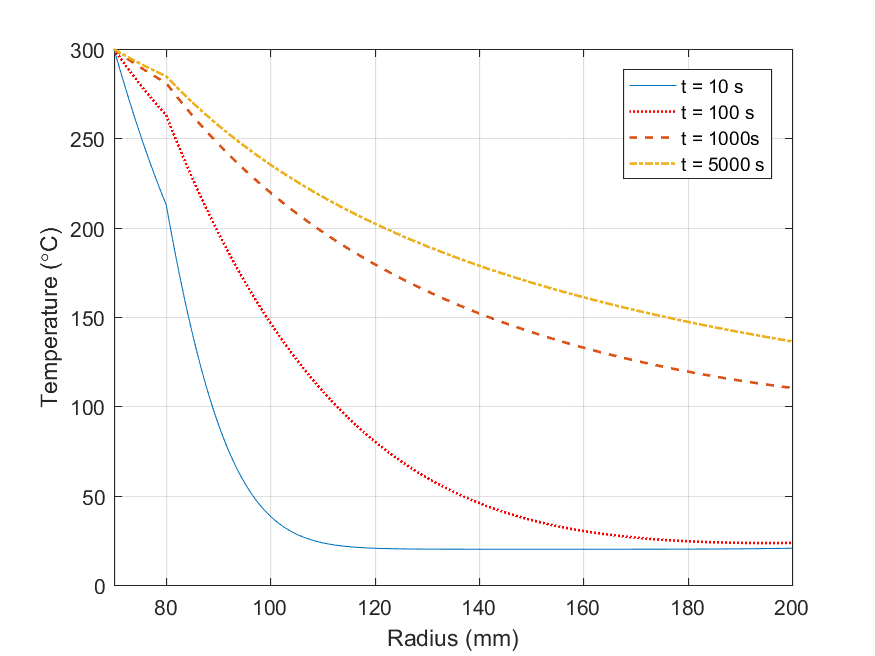
\includegraphics[width=100mm]{TempDistribution} 
\caption{Radial Temperature Distribution of Spherical Pressure Vessel\label{fig:1}}
\end{figure}\\\\
It can be seen in Figure~\ref{fig:1} that the temperature starts at the inner surface where the heat source is located, at 300 $^{\circ}{C}$ and decreases to $\sim{136}$ $^{\circ}{C}$ at the outer after 5,000 seconds (a little longer than 1.25 hours). The temperature decreases much slower throughout the tungsten carbide due to it's thermal conductivity being twice that of steel and the from being insulated by the steel. The temperature decreases much more rapidly after the interface of the two materials, and heat diffuses out to the surroundings due to convective heat transfer. The temperature of the outer surface never reaches ambient temperature at steady state due to the heat source, and the wall thickness being so small. The increase in temperature over time is shown below.
\begin{figure}[!htbp]
\centering 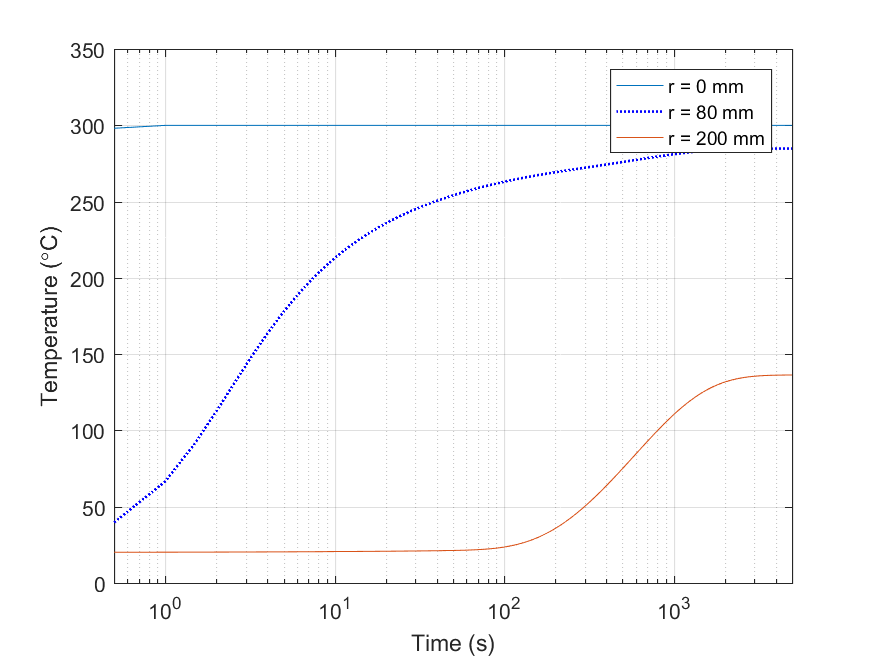
\includegraphics[width=100mm]{TempDistribution_Time}
\caption{Temperature vs. Time at Various Radial Locations \label{fig:2}}
\end{figure}
The temperature at the interface of the material begins increasing almost immediately, and increases to $\sim250~ ^{\circ}{C}$ within a minute and reaches approximate steady state of $\sim282-285~ ^{\circ}{C}$ within the first half hour to one hour. The temperature of the outer surface does not begin increasing until roughly two minutes after the heat source is turned on, and reaches steady state of $136~^{\circ}{C}$ after roughly one hour of heating. The plot shows the time it takes for the heat to transfer from the inner surface to the outer surface. 
\pagebreak
The 2D representation of the temperature distribution throughout the pressure vessel is given in Figure \ref{fig:3} below. 
\begin{figure}[!htbp]
\centering 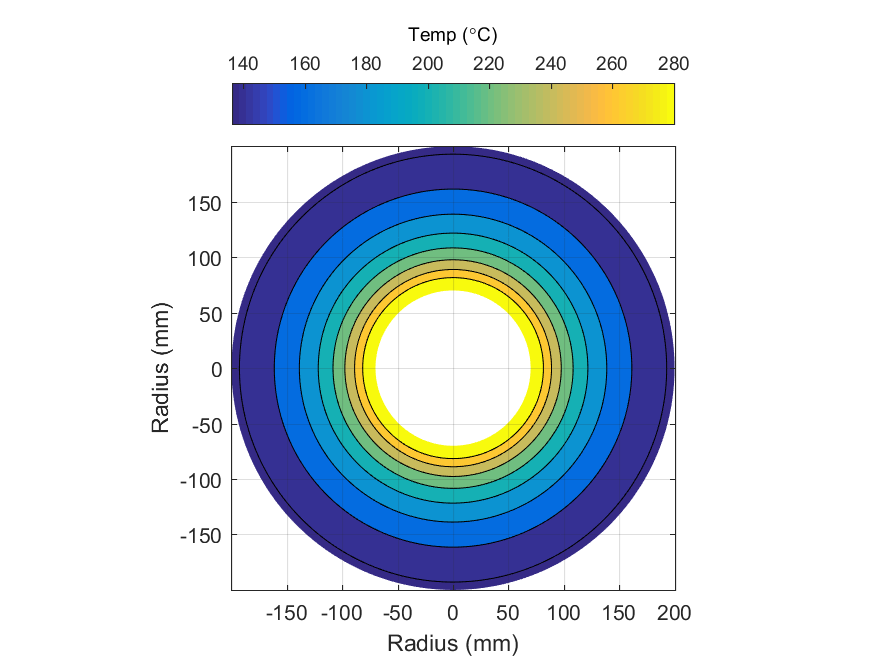
\includegraphics[width=125mm]{2D_TempDistribution}
\caption{2D Radial Temperature Distribution Visualization of the Pressure Vessel}\label{fig:3}
\end{figure}\\
As seen in Figure \ref{fig:3}, the entire inner wall of the vessel is at the maximum temperature of $300~^{\circ}{C}$ and the heat diffuses outward to the outer wall and ultimately the surroundings, leaving the outer wall at $136~^{\circ}{C}$. It's easy to visualize the temperature becoming cooler as you move radially through the sphere. 

\subsection{Mechanical Response}
Not only does the temperature increase throughout the pressure vessel, but the this increase in temperature results in thermal stresses as well. The expansion (radial and azimuthal displacements) cause stresses and strains throughout the pressure vessel wall. The boundary conditions imposed for the mechanical solution were
\begin{enumerate}
\centering
\item $S_{rr} = 0$ for $r = r_{inner}$
\item $S_{rr} = 0$ for $r = r_{outer}$
\item $u = u$ for the interface of the two different materials.
\end{enumerate}
where $u$ is the displacement of the material and $S_{rr}$ denotes the radial stresses throughout the pressure vessel. The following figures show the stress distribution throughout the pressure vessel.
\begin{figure}[!htbp]
\centering 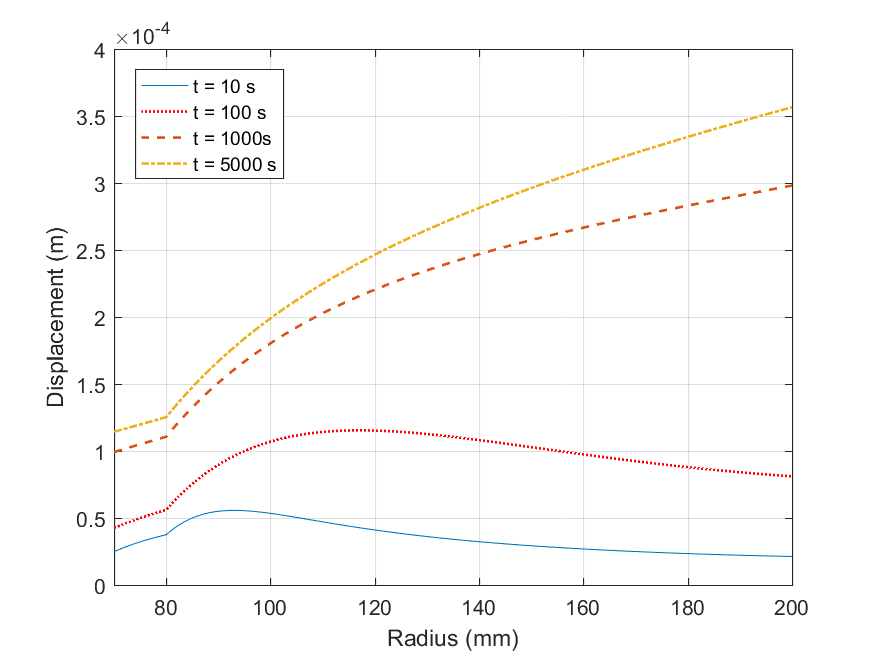
\includegraphics[width=110mm]{Displacement}
\caption{Displacement Throughout the Spherical Pressure Vessel}\label{fig:4}
\end{figure}
The displacement throughout the walls increases slowly throughout the tungsten carbide and increases much more rapidly through the steel due to the steel having a much smaller Young's Modulus. The displacement as a function of time is shown in Figure \ref{fig:5}.
\begin{figure}[!htbp]
\centering 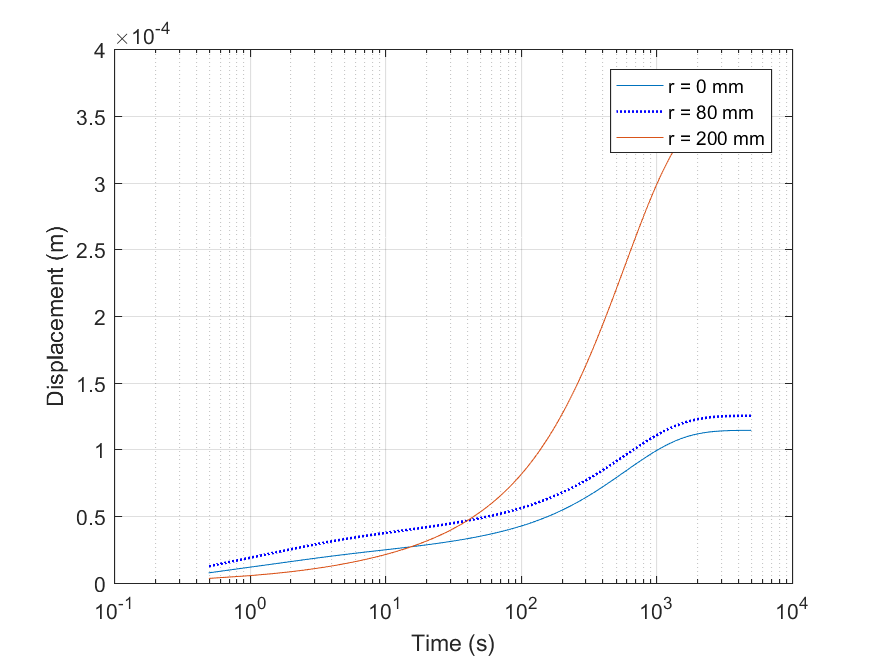
\includegraphics[width=100mm]{Displacement_Time}
\caption{Displacement at Various Times}\label{fig:5}
\end{figure}
It can be seen in Figure \ref{fig:5} that the largest displacement occurs at the outer wall, and is roughly $3.5e-4~m$ or $0.35~mm$. The 2D representation of the displacement is shown below.
\begin{figure}[!htbp]
\centering 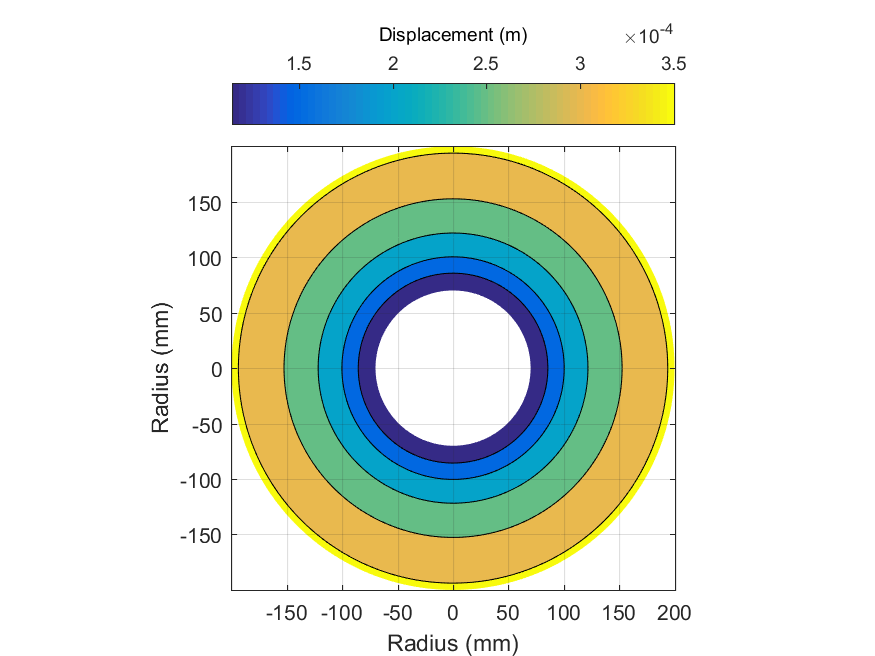
\includegraphics[width=125mm]{2D_Displacement}
\caption{2D Displacement Visualization}\label{fig:6}
\end{figure}
It is much easier to visualize the displacements with the 2D representation. From this representation, the behavior of displacements are shown in a simple manner. The displacements discussed result in radial and azimuthal stresses. The following figures represent the radial and azimuthal stress distributions along with a 2D representation of the stress. 
\begin{figure}[!htbp]
\centering \includegraphics[width=100mm]{S_rr}
\caption{Radial Stress Distribution Throughout the Pressure Vessel}\label{fig:7}
\end{figure}\\\\
The radial stress is a result of the expansion of the two materials. It can be seen in \ref{fig:7} that the stress in tungsten carbide increases linearly to a maximum of $\sim 7.5~Pa$ and then reaches a point where it begins to decrease. The radial stress decreases very rapidly throughout the steel material. One should also note that there is not a discontinuity in the stress at the interface of the material. This is due to the boundary condition imposed where the radial stress has to be equal to the left and right of the interface. 
\begin{figure}[!htbp]
\centering \includegraphics[width=125mm]{2D_RadialStress}
\caption{2D Radial Stress Visualization}\label{fig:8}
\end{figure}\\
The 2D radial stress shown in Figure \ref{fig:8} shows how the stress goes from $\sim 700~MPa$ to roughly $0~ MPa$. 
\begin{figure}[!htbp]
\centering 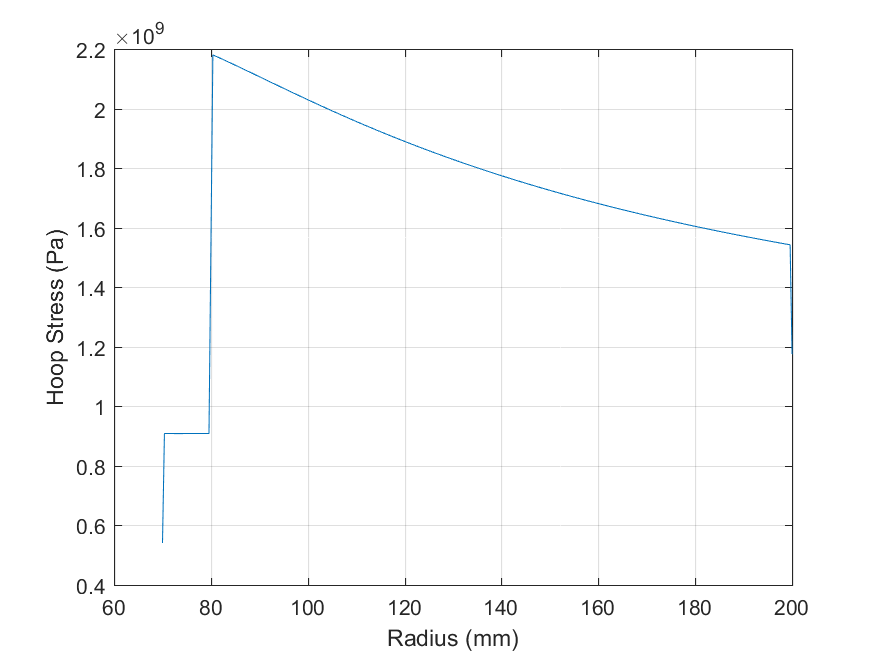
\includegraphics[width=100mm]{S_thth}
\caption{Hoop Stress Distribution Throughout the Pressure Vessel}\label{fig:9}
\end{figure}\\
\begin{figure}[!htbp]
\centering 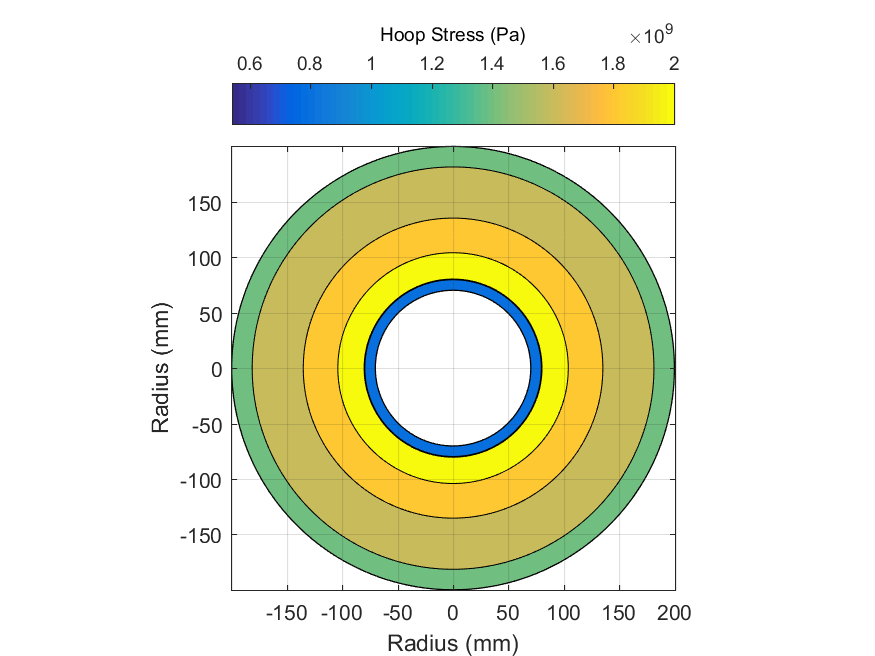
\includegraphics[width=125mm]{2D_HoopStress}
\caption{2D Hoop Stress Visualization}\label{fig:10}
\end{figure}\\
The Hoop stress distribution shown in Figures \ref{fig:9} and \ref{fig:10} show a discontinuity in the material at the interface. This is because the stresses are not equal at this point, therefore, the stress is much higher in the steel than in the tungsten carbide. This can be seen in the rapid increase in stress right along the interface of the two materials.  
\pagebreak
\vspace{-2pt}
\section{Conclusions}
\vspace{-2pt}

The implicit finite difference method was utilized to determine the temperature distribution of the pressure vessel using the one dimensional heat conduction equation in spherical coordinates. Since the implicit method was used, the solution took the form of $\utilde{A}\underline{u} = \underline{b}$, where $\utilde{A}$ is the coefficient matrix and \underline{b} is the known temperature vector. The same techniques were applied to determine the displacements throughout the pressure vessel. Once all of the displacements were determined, they were plugged into equations \eqref{eqn:13} and \eqref{eqn:17}.\\
\\
It was shown that the energy diffuses through the tungsten carbide much slower than that of the steel material. Steel also transfers heat better and has a much smaller Young's Modulus, therefore, the steel expands much more than the tungsten carbide; almost three times as much. Although the steel expands more, the tungsten carbide has much higher radial stresses which leads to higher azimuthal stresses. 

\ack I am fairly new to LaTex so I apologize if the formatting of the figures are not in a nice manner. They are not falling in the order they were called, and I know there is a way to fix this issue but I'd have to spend some more time learning the software.\\

\begin{thebibliography}{9}
\bibitem{R1} Cherukuri, Harish. n.d. "Computation Methods in Engineering (Fall 2016)." https://sites.google.com/a/uncc.edu/cme2016/.
\end{thebibliography}


\end{document}
